% creator: ilyakooo0
% extra credit: dashared
% version: 1.0.1

\PassOptionsToPackage{main=russian,english}{babel}

\documentclass{../TechDoc}
\usepackage{pmboxdraw}

\title{Генератор данных для аналитического бенчмарка СУБД TPC-H}
\author{Студент БПИ225}{Дергоусов М.А}
\academicTeacher{Профессор департамента программной инженерии ФКН НИУ ВШЭ}{Шилов В.В}

\documentTitle{Пояснительная записка}
\documentCode{RU.17701729.11.03-01 81 01-1}

\definecolor{listingbg}{gray}{0.96}
\definecolor{listingkw}{RGB}{0,74,140}
\definecolor{listingtype}{RGB}{120,78,0}
\definecolor{listingcomment}{RGB}{0,120,60}
\definecolor{listingstring}{RGB}{163,21,21}
\renewcommand{\lstlistingname}{Листинг}
\DeclareCaptionLabelSeparator{listinghyphen}{ - }
\captionsetup[lstlisting]{
    font=small,
    labelfont=bf,
    justification=raggedright,
    singlelinecheck=false,
    skip=6pt,
    labelsep=listinghyphen
}
\captionsetup[figure]{
    labelsep=listinghyphen
}

\DeclareRobustCommand{\srcref}[1]{\mbox{\hyperlink{src:#1}{[#1]}}}

\lstdefinelanguage{DSS}{
    sensitive=false,
    morekeywords={BEGIN,END,COUNT,begin,end,count},
    morekeywords=[2]{grammar,np,vp,articles,nouns,verbs,adverbs,prepositions},
    morekeywords=[3]{N,V,P,T,J,D,X},
    morecomment=[l]{\#}
}

\lstdefinestyle{dsslisting}{
    language=DSS,
    basicstyle=\ttfamily\footnotesize,
    keywordstyle=\color{listingkw}\bfseries,
    keywordstyle=[2]\color{listingtype}\bfseries,
    keywordstyle=[3]\color{listingstring}\bfseries,
    commentstyle=\color{listingcomment}\itshape,
    breaklines=true,
    columns=fullflexible,
    showstringspaces=false,
    keepspaces=true,
    frame=single,
    framerule=0.4pt,
    rulecolor=\color{black},
    backgroundcolor=\color{listingbg},
    framesep=6pt,
    captionpos=b,
    aboveskip=6pt,
    belowskip=10pt
}

\lstdefinelanguage{DuckDBPlan}{
    sensitive=false,
    alsoletter={_},
    morekeywords={EXPLAIN,SELECT,FROM,WHERE,GROUP,BY,ORDER,SUM,AVG,COUNT,AS,DATE,CALL},
    morekeywords=[2]{OPTIMIZED_LOGICAL_PLAN,ORDER_BY,PROJECTION,AGGREGATE,FILTER,SCHENGEN_SCAN},
    morecomment=[l]{--},
    morestring=[b]'
}

\lstdefinestyle{duckdbplanlisting}{
    language=DuckDBPlan,
    basicstyle=\ttfamily\footnotesize,
    keywordstyle=\color{listingkw}\bfseries,
    keywordstyle=[2]\color{listingtype}\bfseries,
    commentstyle=\color{listingcomment}\itshape,
    stringstyle=\color{listingstring},
    breaklines=false,
    columns=fixed,
    showstringspaces=false,
    keepspaces=true,
    frame=single,
    framerule=0.4pt,
    rulecolor=\color{black},
    backgroundcolor=\color{listingbg},
    framesep=6pt,
    captionpos=b,
    aboveskip=6pt,
    belowskip=10pt,
    literate=
        {┌}{{\textSFi}}1
        {┐}{{\textSFiii}}1
        {└}{{\textSFii}}1
        {┘}{{\textSFiv}}1
        {─}{{\textSFx}}1
        {│}{{\textSFxi}}1
        {┬}{{\textSFvi}}1
        {┴}{{\textSFvii}}1
}

\begin{document}
    \maketitle

    \tableofcontents

    \section{Введение}

\subsection{Наименование разработки}

\subsubsection{Наименование разработки на русском языке}

<<Генератор данных для аналитического бенчмарка СУБД TPC-H>>.

\subsubsection{Наименование разработки на английском языке}

<<Data Generator for the TPC-H Analytical DBMS Benchmark>>.

\subsubsection{Условное обозначение темы разработки}

\texttt{Schengen}.

Исходный код программы размещается в репозитории \texttt{Schengen}
\srcref{10}.

\subsection{Документы, являющиеся основанием для разработки}

Разработка ведется на основании следующих документов:
\begin{enumerate}
    \item учебный план подготовки бакалавров по направлению 09.03.04
    <<Программная инженерия>> федерального государственного автономного
    образовательного учреждения высшего образования Национальный
    исследовательский университет <<Высшая школа экономики>>;
    \item утвержденная академическим руководителем образовательной программы
    тема выпускной квалификационной работы <<Генератор данных для аналитического
    бенчмарка СУБД TPC-H>>;
    \item техническое задание \texttt{RU.17701729.04.03-01 ТЗ 01-1},
    разработанное в рамках выполнения выпускной квалификационной работы.
\end{enumerate}

\subsection{Предпосылки разработки}

Необходимость разработки определяется тем, что существующие генераторы данных
TPC-H \srcref{1} либо ориентированы на вывод в строковые файлы
\texttt{tbl}/\texttt{csv} \srcref{4}, либо не учитывают требований современной
инфраструктуры аналитического хранения и обработки данных, использующей
колонoчные форматы \texttt{Parquet} \srcref{5} и \texttt{ORC} \srcref{6}, а
также табличные слои lakehouse-платформ \srcref{7}.

В практических сценариях разработки и исследования аналитических систем
требуется средство, обеспечивающее детерминированную генерацию таблиц TPC-H
\srcref{1}, прямую запись в современные колонoчные форматы \texttt{Parquet}
\srcref{5}, \texttt{ORC} \srcref{6}, \texttt{Lance} \srcref{8} и
\texttt{Vortex} \srcref{9}, поддержку параллельного формирования партиций в
духе систем параллельной обработки данных \srcref{2} и возможность работы как
с локальной файловой системой, так и с \texttt{S3}-совместимыми хранилищами.

    \section{Назначение и область применения}

\subsection{Назначение программы}

Назначением программы является формирование синтетических данных аналитического
бенчмарка TPC-H \srcref{1} с заданным масштабом генерации и сохранением результатов в
форматах, пригодных для непосредственного использования в современных
аналитических системах и подсистемах хранения данных.

Программа предназначена для детерминированной генерации таблиц набора TPC-H,
их представления в колонoчной форме Apache Arrow \srcref{3} и записи результата в
поддерживаемые форматы хранения без промежуточного этапа ручной конвертации.
В отличие от традиционных генераторов, ограниченных выводом в
\texttt{tbl}/\texttt{csv} \srcref{4}, разрабатываемая программа обеспечивает
прямое формирование данных в форматах \texttt{Parquet} \srcref{5},
\texttt{ORC} \srcref{6}, \texttt{Lance} \srcref{8} и \texttt{Vortex}
\srcref{9} и допускает запись как на
локальную файловую систему, так и в \texttt{S3}-совместимые объектные
хранилища.

\subsection{Область применения программы}

Программа может применяться при разработке, испытаниях и исследовании
аналитических СУБД и OLAP-движков \srcref{2}, lakehouse-платформ,
подсистем хранения данных и
других программных средств, работающих с большими объемами колонoчных данных.

Основными областями применения программы являются:
\begin{enumerate}
    \item подготовка воспроизводимых наборов данных для функционального и
    нагрузочного тестирования аналитических систем;
    \item исследование характеристик различных форматов хранения и стратегий
    записи данных;
    \item проверка корректности работы систем чтения, сериализации и обработки
    колонoчных данных;
    \item проведение сравнительных экспериментов, связанных с локальным и
    удаленным размещением аналитических наборов данных.
\end{enumerate}

Программа ориентирована на использование разработчиками, исследователями,
инженерами по тестированию и иными специалистами, которым требуется быстрое,
детерминированное и масштабируемое получение данных набора TPC-H в форме,
непосредственно пригодной для дальнейшего анализа и эксплуатации.

    \section{Технические характеристики}

\subsection{Постановка задачи, применяемые методы, допущения и ограничения}

Задача разработки заключается в создании программы, обеспечивающей генерацию
таблиц аналитического бенчмарка TPC-H \srcref{1} в соответствии с правилами и
распределениями эталонной спецификации с возможностью выбора масштаба
генерации, состава формируемых таблиц, формата хранения результата и способа
организации записи выходных данных.

При разработке применяются методы детерминированной генерации данных на основе
фиксированных последовательностей случайных значений, используемых в
классическом генераторе TPC-H \srcref{1}, методы колонoчного представления
данных в оперативной памяти \srcref{3}, а также методы разбиения таблиц на
партиции с
последующим параллельным формированием и сериализацией результата. Для
обеспечения совместимости с современными аналитическими форматами в качестве
внутреннего представления используются колонoчные структуры данных Apache
Arrow \srcref{3}.

В качестве основных допущений и ограничений принимается, что программа работает
с фиксированным составом таблиц набора TPC-H и использует заданные спецификацией
схемы, распределения и правила вычисления зависимых атрибутов. Поддерживаемые
форматы хранения и конкретные параметры сериализации определяются конфигурацией
сборки программы и набором подключенных форматных библиотек \texttt{Parquet}
\srcref{5}, \texttt{ORC} \srcref{6}, \texttt{Lance} \srcref{8} и
\texttt{Vortex} \srcref{9}.
Возможность записи в удаленные хранилища определяется доступностью
соответствующей файловой подсистемы и корректностью указанного URI.

\subsection{Описание алгоритма и функционирования программы}

\subsubsection{Общая идея алгоритма}

Функционирование программы организовано как последовательность этапов выбора
сценария генерации, формирования таблиц и записи результата.

На первом этапе программа обрабатывает параметры командной строки, определяющие
масштаб генерации, состав таблиц, формат вывода и путь размещения результата.
После этого выполняется регистрация метаданных таблиц и выбирается требуемый
драйвер сериализации.

На втором этапе для каждой выбранной таблицы определяется объем данных и схема
разбиения на логические партиции. Далее для каждой партиции запускается
генератор, формирующий значения атрибутов по детерминированным правилам TPC-H.

На третьем этапе сгенерированные значения накапливаются и объединяются в батчи
для увеличения пропускной способности. После этого батчи передаются слою
сериализации, который сохраняет результат в требуемом формате хранения.

\subsubsection{Генерация значений и использование текстового пула}

Формирование значений атрибутов основано на детерминированных последовательностях
случайных чисел с фиксированными начальными значениями. За счет этого при
одинаковых параметрах запуска программа воспроизводит один и тот же набор
данных независимо от числа партиций и конфигурации параллельного выполнения.

Для числовых атрибутов используются ограниченные генераторы целых значений. Они
применяются, например, при получении размеров деталей, балансов клиентов и
поставщиков, скидок, налогов, датовых смещений и других величин, для которых
спецификацией TPC-H задан конечный диапазон допустимых значений. Для больших
диапазонов ключей используется расширенный вариант генерации, допускающий работу
с 64-разрядными значениями.

Для строковых атрибутов применяются несколько способов формирования значения.
Значения из фиксированных словарей, например сегменты рынка, приоритеты заказов,
типы деталей, инструкции отгрузки и режимы доставки, выбираются из взвешенных
распределений. Имена деталей формируются как последовательности токенов, а
адреса строятся как алфавитно-цифровые строки переменной длины. Телефонные
номера вычисляются из ключа страны и случайных локальных компонент.

Генерация текстовых атрибутов в TPC-H задается набором распределений из файла
\texttt{dists.dss} \srcref{1}. Каждый блок содержит имя распределения и число
элементов \texttt{COUNT}. Далее приводится список токенов с соответствующими
весами; вес определяет относительную частоту выбора токена.

\begin{lstlisting}[style=dsslisting,caption={Общий вид распределения}]
# <token> | <weight> # comment

BEGIN articles
COUNT|3
the|50
a|20
an|5
END articles
\end{lstlisting}

Распределение \texttt{grammar} задает верхнеуровневую схему предложения.
Символы \texttt{N}, \texttt{V}, \texttt{P} и \texttt{T} обозначают именную
группу, глагольную группу, предложную группу и знак завершения предложения.

\begin{lstlisting}[style=dsslisting,caption={Верхнеуровневая грамматика предложения}]
###
# grammar
# first level grammar. N=noun phrase, V=verb phrase,
# P=prepositional phrase, T=sentence termination
##
BEGIN grammar
COUNT|5
N V T|3
N V P T|3
N V N T|3
N P V N T|1
N P V P T|1
END grammar
\end{lstlisting}

Далее нетерминальные символы раскрываются через распределения \texttt{np} и
\texttt{vp}, которые определяют внутреннюю форму именной и глагольной групп.

\begin{lstlisting}[style=dsslisting,caption={Раскрытие именной и глагольной групп}]
###
# NP
BEGIN np
COUNT|4
N|10
J N|20
J, J N|10
D J N|50
END np

###
# VP
BEGIN vp
COUNT|4
V|30
X V|1
V D|40
X V D|1
END vp
\end{lstlisting}

Терминальные символы подставляются из словарей отдельных частей речи, например
\texttt{nouns} и \texttt{verbs}.

\begin{lstlisting}[style=dsslisting,caption={Словари терминальных токенов}]
BEGIN nouns
COUNT|45
packages|40
requests|40
accounts|40
deposits|40
foxes|20
ideas|20
END nouns

BEGIN verbs
COUNT|40
sleep|20
wake|20
are|20
cajole|20
haggle|20
END verbs
\end{lstlisting}

Из получаемых предложений заранее формируется \texttt{TextPool} - общий
текстовый буфер. При генерации конкретного комментария программа выбирает в нем
смещение и длину фрагмента, после чего использует соответствующий срез как
значение атрибута. Такой подход уменьшает накладные расходы при генерации
длинных текстовых полей. Для некоторых таблиц, например \texttt{supplier},
поверх выбранного текста дополнительно может применяться модификация по правилу
\texttt{BBB}\footnote{Правило \texttt{BBB} применяется при формировании
атрибута \texttt{s\_comment} таблицы \texttt{supplier}: в текст комментария
вставляется подстрока \texttt{Customer Complaints} или
\texttt{Customer Recommends} \srcref{1}.}, предусмотренному спецификацией
TPC-H \srcref{1}.

\begin{figure}[h]
\centering
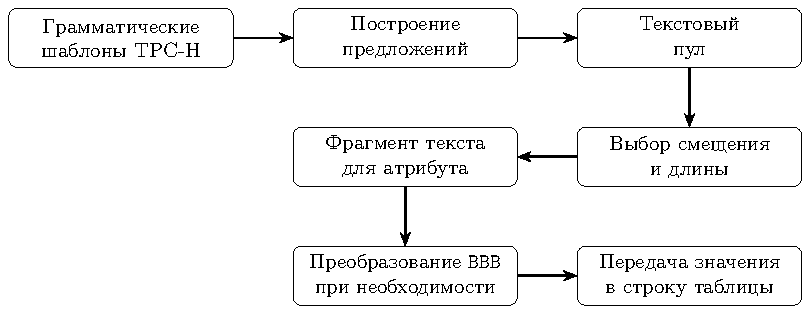
\includegraphics[width=0.92\textwidth]{image/textpool-diagram.pdf}
\caption{Схема формирования текстовых атрибутов на основе пула текста}
\end{figure}

\subsubsection{Формирование таблиц набора данных}

Генерация каждой таблицы выполняется отдельным модулем. Для всех таблиц
используются фиксированные схемы и согласованные правила формирования ключей и
зависимых атрибутов.

\renewcommand{\arraystretch}{1.1}

\paragraph{Таблица \texttt{region}}
\begin{center}
\small
\begin{tabular}{|p{0.18\textwidth}|p{0.10\textwidth}|p{0.58\textwidth}|}
\hline
\textbf{Атрибут} & \textbf{Ключ} & \textbf{Правило формирования} \\
\hline
\texttt{r\_regionkey} & PK & Последовательная нумерация строк, начиная с нуля. \\
\hline
\texttt{r\_name} &  & Выбирается из фиксированного справочника регионов TPC-H. \\
\hline
\texttt{r\_comment} &  & Выбирается из пула текста \texttt{TextPool}. \\
\hline
\end{tabular}
\end{center}

\paragraph{Таблица \texttt{nation}}
\begin{center}
\small
\begin{tabular}{|p{0.18\textwidth}|p{0.10\textwidth}|p{0.58\textwidth}|}
\hline
\textbf{Атрибут} & \textbf{Ключ} & \textbf{Правило формирования} \\
\hline
\texttt{n\_nationkey} & PK & Последовательная нумерация строк, начиная с нуля. \\
\hline
\texttt{n\_name} &  & Выбирается из предопределенного справочника наций. \\
\hline
\texttt{n\_regionkey} & FK & Вычисляется по таблице наций и весам распределения регионов, заданным спецификацией TPC-H. \\
\hline
\texttt{n\_comment} &  & Выбирается из пула текста \texttt{TextPool}. \\
\hline
\end{tabular}
\end{center}

\paragraph{Таблица \texttt{supplier}}
\begin{center}
\small
\begin{tabular}{|p{0.18\textwidth}|p{0.10\textwidth}|p{0.58\textwidth}|}
\hline
\textbf{Атрибут} & \textbf{Ключ} & \textbf{Правило формирования} \\
\hline
\texttt{s\_suppkey} & PK & Номер строки с единичным смещением. \\
\hline
\texttt{s\_name} &  & Формируется по шаблону \texttt{Supplier\#\%09d}. \\
\hline
\texttt{s\_address} &  & Формируется как алфавитно-цифровая строка переменной длины. \\
\hline
\texttt{s\_nationkey} & FK & Выбирается из допустимого диапазона ключей наций. \\
\hline
\texttt{s\_phone} &  & Вычисляется из ключа страны и случайных локальных компонент. \\
\hline
\texttt{s\_acctbal} &  & Генерируется как ограниченное числовое значение и переводится в денежный формат. \\
\hline
\texttt{s\_comment} &  & Выбирается из пула текста; при выполнении условия может модифицироваться по правилу \texttt{BBB}. \\
\hline
\end{tabular}
\end{center}

\paragraph{Таблица \texttt{part}}
\begin{center}
\small
\begin{tabular}{|p{0.18\textwidth}|p{0.10\textwidth}|p{0.58\textwidth}|}
\hline
\textbf{Атрибут} & \textbf{Ключ} & \textbf{Правило формирования} \\
\hline
\texttt{p\_partkey} & PK & Последовательная нумерация строк с единичным смещением. \\
\hline
\texttt{p\_name} &  & Формируется как последовательность токенов из словаря цветов. \\
\hline
\texttt{p\_mfgr} &  & Строится по номеру производителя. \\
\hline
\texttt{p\_brand} &  & Вычисляется по номеру производителя и дополнительному номеру бренда. \\
\hline
\texttt{p\_type} &  & Выбирается из словаря типов деталей. \\
\hline
\texttt{p\_size} &  & Генерируется из ограниченного числового диапазона. \\
\hline
\texttt{p\_container} &  & Выбирается из словаря контейнеров. \\
\hline
\texttt{p\_retailprice} &  & Детерминированно вычисляется по ключу детали. \\
\hline
\texttt{p\_comment} &  & Выбирается из пула текста \texttt{TextPool}. \\
\hline
\end{tabular}
\end{center}

\paragraph{Таблица \texttt{partsupp}}
\begin{center}
\small
\begin{tabular}{|p{0.18\textwidth}|p{0.10\textwidth}|p{0.58\textwidth}|}
\hline
\textbf{Атрибут} & \textbf{Ключ} & \textbf{Правило формирования} \\
\hline
\texttt{ps\_partkey} & FK & Соответствует текущей детали. \\
\hline
\texttt{ps\_suppkey} & FK & Вычисляется как детерминированное отображение пары <<ключ детали, номер поставщика>>; для каждой детали формируются четыре поставщика. \\
\hline
\texttt{ps\_availqty} &  & Генерируется из ограниченного диапазона доступного количества. \\
\hline
\texttt{ps\_supplycost} &  & Генерируется из ограниченного диапазона и переводится в денежный формат. \\
\hline
\texttt{ps\_comment} &  & Выбирается из пула текста \texttt{TextPool}. \\
\hline
\end{tabular}
\end{center}

\paragraph{Таблица \texttt{customer}}
\begin{center}
\small
\begin{tabular}{|p{0.18\textwidth}|p{0.10\textwidth}|p{0.58\textwidth}|}
\hline
\textbf{Атрибут} & \textbf{Ключ} & \textbf{Правило формирования} \\
\hline
\texttt{c\_custkey} & PK & Последовательная нумерация строк с единичным смещением. \\
\hline
\texttt{c\_name} &  & Формируется по шаблону \texttt{Customer\#\%09d}. \\
\hline
\texttt{c\_address} &  & Формируется как алфавитно-цифровая строка переменной длины. \\
\hline
\texttt{c\_nationkey} & FK & Выбирается из допустимого диапазона ключей наций. \\
\hline
\texttt{c\_phone} &  & Вычисляется из ключа страны и случайных локальных компонент. \\
\hline
\texttt{c\_acctbal} &  & Генерируется как ограниченное числовое значение и переводится в денежный формат. \\
\hline
\texttt{c\_mktsegment} &  & Выбирается из словаря сегментов рынка. \\
\hline
\texttt{c\_comment} &  & Выбирается из пула текста \texttt{TextPool}. \\
\hline
\end{tabular}
\end{center}

\paragraph{Таблица \texttt{orders}}
\begin{center}
\small
\begin{tabular}{|p{0.18\textwidth}|p{0.10\textwidth}|p{0.58\textwidth}|}
\hline
\textbf{Атрибут} & \textbf{Ключ} & \textbf{Правило формирования} \\
\hline
\texttt{o\_orderkey} & PK & Строится по разреженной схеме из порядкового номера заказа. \\
\hline
\texttt{o\_custkey} & FK & Выбирается из диапазона клиентов с исключением недопустимых ключей. \\
\hline
\texttt{o\_orderstatus} &  & Определяется по числу отгруженных позиций заказа. \\
\hline
\texttt{o\_totalprice} &  & Вычисляется как агрегат по позициям соответствующего заказа. \\
\hline
\texttt{o\_orderdate} &  & Генерируется в допустимом диапазоне дат TPC-H. \\
\hline
\texttt{o\_orderpriority} &  & Выбирается из словаря приоритетов заказов. \\
\hline
\texttt{o\_clerk} &  & Формируется по шаблону \texttt{Clerk\#\%09d}. \\
\hline
\texttt{o\_shippriority} &  & Имеет фиксированное значение \texttt{0}. \\
\hline
\texttt{o\_comment} &  & Выбирается из пула текста \texttt{TextPool}. \\
\hline
\end{tabular}
\end{center}

\paragraph{Таблица \texttt{lineitem}}
\begin{center}
\small
\begin{tabular}{|p{0.18\textwidth}|p{0.10\textwidth}|p{0.58\textwidth}|}
\hline
\textbf{Атрибут} & \textbf{Ключ} & \textbf{Правило формирования} \\
\hline
\texttt{l\_orderkey} & FK & Согласован с ключом соответствующего заказа. \\
\hline
\texttt{l\_partkey} & FK & Выбирается из диапазона ключей деталей. \\
\hline
\texttt{l\_suppkey} & FK & Вычисляется по паре <<ключ детали, номер поставщика>>. \\
\hline
\texttt{l\_linenumber} &  & Задает порядковый номер позиции внутри заказа. \\
\hline
\texttt{l\_quantity} &  & Генерируется из ограниченного числового диапазона. \\
\hline
\texttt{l\_extendedprice} &  & Вычисляется по цене детали и количеству. \\
\hline
\texttt{l\_discount} &  & Генерируется как процент скидки из ограниченного диапазона. \\
\hline
\texttt{l\_tax} &  & Генерируется как процент налога из ограниченного диапазона. \\
\hline
\texttt{l\_returnflag} &  & Определяется по отношению даты получения к текущей календарной отметке TPC-H. \\
\hline
\texttt{l\_linestatus} &  & Определяется по отношению даты отгрузки к текущей календарной отметке TPC-H. \\
\hline
\texttt{l\_shipdate} &  & Вычисляется как смещение относительно даты заказа. \\
\hline
\texttt{l\_commitdate} &  & Вычисляется как смещение относительно даты заказа. \\
\hline
\texttt{l\_receiptdate} &  & Вычисляется как смещение относительно даты отгрузки. \\
\hline
\texttt{l\_shipinstruct} &  & Выбирается из словаря инструкций по отгрузке. \\
\hline
\texttt{l\_shipmode} &  & Выбирается из словаря режимов доставки. \\
\hline
\texttt{l\_comment} &  & Выбирается из пула текста \texttt{TextPool}. \\
\hline
\end{tabular}
\end{center}

\subsubsection{Сериализация результатов}

После формирования батчей данные передаются в драйвер выбранного формата
хранения. Слой сериализации отделен от слоя генерации, поэтому одна и та же
схема формирования таблиц может использоваться для нескольких форматов вывода.

\paragraph{Форматы Parquet и ORC.}
Форматы \texttt{Parquet} \srcref{5} и \texttt{ORC} \srcref{6} являются
основными колонoчными
форматами, поддерживаемыми программой. Для них используются две стратегии
записи.

При стратегии \texttt{parallel-files} каждая логическая партиция генерируется
отдельным рабочим потоком и записывается в собственный файл. Таким образом,
для одной таблицы формируется каталог, содержащий набор файлов партиций.
Линейный порядок результата при этом задается номерами партиций: каждая
партиция соответствует своему непрерывному диапазону строк, а номер партиции
фиксируется в имени файла, что позволяет однозначно восстановить общий порядок
таблицы при последующем чтении.

При стратегии \texttt{single-file-ordered} генерация партиций также может
выполняться параллельно, однако их батчи передаются из рабочих потоков через
ограниченную очередь \texttt{MPSC}\footnote{\texttt{MPSC}
(\textit{multi-producer, single-consumer}) - очередь с несколькими
источниками и одним потребителем.} одному потоку записи. На стороне
потребителя
батчи временно буферизуются по номеру партиции и выгружаются в файл только
тогда, когда для записи готова очередная ожидаемая партиция. За счет этого
порядок данных в итоговом файле эквивалентен последовательной обработке
партиций с номерами от \texttt{1} до \texttt{N}, несмотря на параллельную
генерацию.

\begin{figure}[h]
\centering
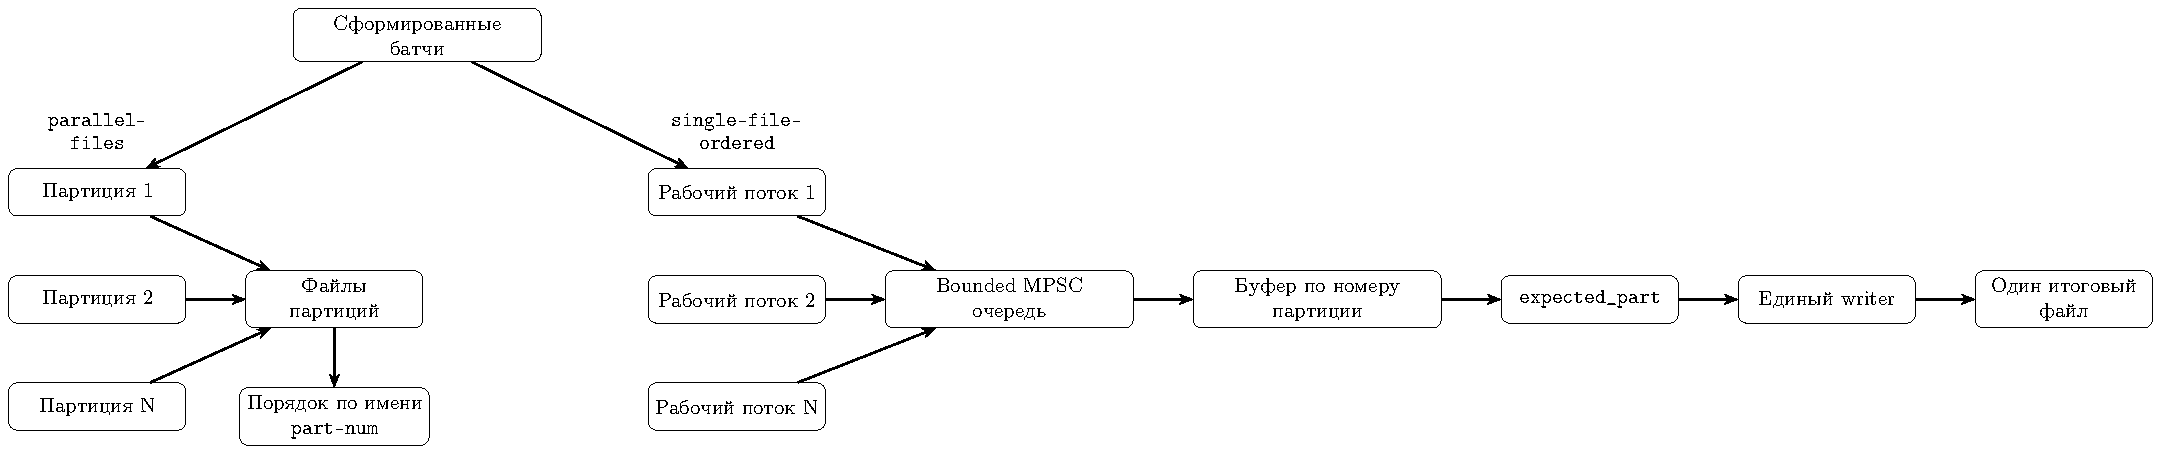
\includegraphics[width=\textwidth]{image/serialization-diagram.pdf}
\caption{Схема ручного упорядочения партиций для форматов Parquet и ORC}
\end{figure}

\paragraph{Форматы Lance и Vortex.}
Для форматов \texttt{Lance} \srcref{8} и \texttt{Vortex} \srcref{9}
используется другой
подход.
Схема таблицы, батчи и границы входных партиций передаются в форматно-зависимый
мост через интерфейс Arrow C ABI, после чего дальнейшая организация записи
делегируется рантайму библиотеки соответствующего формата. В отличие от
\texttt{Parquet} и \texttt{ORC}, ручное упорядочение через очередь и буфер по
номеру партиции в данном случае не реализуется на стороне программы.

\subsection{Организация входных и выходных данных}

Входные данные программы представлены параметрами командной строки. К числу
основных входных параметров относятся значение \texttt{scale
factor}\footnote{\texttt{Scale factor} - размер формируемого набора данных в
гигабайтах \srcref{1}.}, перечень формируемых таблиц, формат хранения
результата, путь
или URI вывода, размер колонoчного батча, стратегия записи и
форматно-зависимые параметры сериализации.

Предварительно подготовленные табличные входные данные для работы программы не
требуются. Все словари, распределения, шаблоны текстов и правила вычисления
атрибутов входят в состав программы и используются непосредственно в процессе
генерации.

Выходные данные программы представляют собой сформированные таблицы набора TPC-H
в поддерживаемом формате хранения. Результат может быть организован либо как
набор файлов-партиций, либо как единый файл таблицы, формируемый из нескольких
логических партиций в заранее определенном порядке. Размещение результатов
допускается как на локальных носителях данных, так и в S3-совместимых объектных
хранилищах.

Внутри программы перед сериализацией данные организуются в виде колонoчных
батчей, соответствующих схеме выбранной таблицы. Такой способ организации
входных и выходных данных уменьшает объем промежуточных преобразований и
позволяет непосредственно передавать сформированные батчи в драйверы записи.
Выбранная форма представления согласуется с моделью обмена данных Apache Arrow
\srcref{3}.

\subsection{Состав технических и программных средств}

Подробное описание состава технических и программных средств, а также условий
эксплуатации приведено в документе «Руководство оператора», раздел 2
«Условия выполнения программы».

    \section{Ожидаемые технико-экономические показатели}

\subsection{Сокращение трудоемкости подготовки данных}

Выбранное техническое решение позволяет исключить промежуточный этап
формирования табличных файлов в формате \texttt{tbl/csv} \srcref{4} с
последующей
конвертацией в целевой формат хранения. За счет прямой генерации данных в
поддерживаемые колонoчные форматы \texttt{Parquet} \srcref{5},
\texttt{ORC} \srcref{6}, \texttt{Lance} \srcref{8} и \texttt{Vortex}
\srcref{9} сокращается количество операций, выполняемых при подготовке наборов
данных к нагрузочным испытаниям и исследовательским экспериментам.
Детерминированный характер генерации, предусмотренный спецификацией TPC-H
\srcref{1}, дополнительно упрощает повторное
проведение экспериментов при одинаковых параметрах запуска.

\subsection{Снижение инфраструктурных издержек}

Прямая запись результата в локальную файловую систему и в
\texttt{S3}-совместимые хранилища позволяет отказаться от отдельного конвейера
выгрузки, последующей конвертации и доставки данных в среду выполнения
аналитических запросов. Отсутствие обязательной материализации промежуточных
форматов уменьшает потребность во временном дисковом пространстве и снижает
накладные расходы на подготовку испытательной и исследовательской
инфраструктуры.

\subsection{Расширение вариантов интеграции}

Отделение модуля генерации от слоя сериализации позволяет
использовать программу как встраиваемый источник табличных данных. В этом
режиме таблицы \texttt{TPC-H} формируются непосредственно в оперативной
памяти и передаются потребителю без промежуточной записи на диск. Исходная
реализация генератора представлена в репозитории \texttt{Schengen}
\srcref{10}.

Такой способ интеграции реализован для СУБД DuckDB в отдельном расширении
\srcref{11}. Расширение регистрирует представления таблиц
\texttt{TPC-H}, а обращение к ним приводит к вызову табличной функции
\texttt{SCHENGEN\_SCAN}, получающей данные напрямую из генератора в виде
батчей Apache Arrow \srcref{3}.

\begin{center}
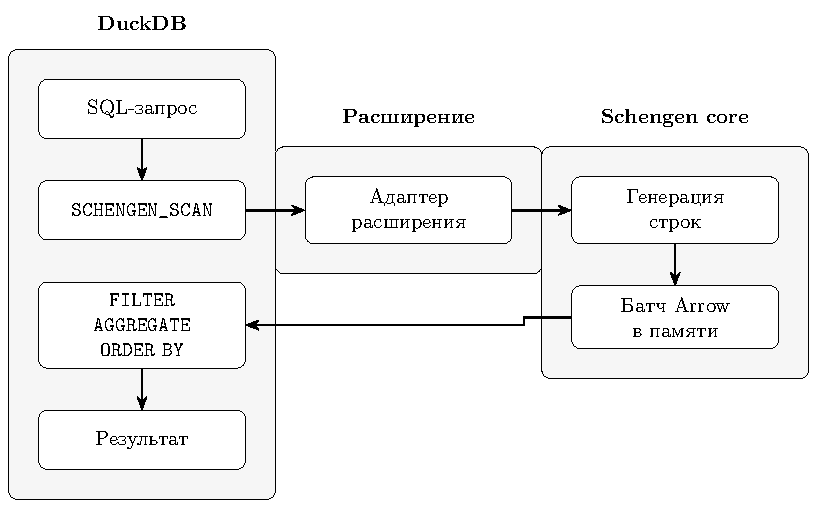
\includegraphics[width=0.78\textwidth]{image/duckdb-integration-diagram.pdf}
\captionof{figure}{Схема интеграции генератора с DuckDB}
\end{center}
\medskip

В листинге 5 приведен пример вывода \texttt{EXPLAIN} DuckDB для запроса
\texttt{TPC-H Q1} \srcref{1}. Наличие оператора \texttt{SCHENGEN\_SCAN} в нижней
части плана показывает, что данные поступают из генератора, а не считываются
из файла.

\begin{lstlisting}[style=duckdbplanlisting,caption={Вывод DuckDB \texttt{EXPLAIN} для запроса \texttt{TPC-H Q1}}]
D EXPLAIN SELECT
    l_returnflag,
    l_linestatus,
    SUM(l_quantity) AS sum_qty,
    SUM(l_extendedprice) AS sum_base_price,
    SUM(l_extendedprice * (1 - l_discount)) AS sum_disc_price,
    SUM(l_extendedprice * (1 - l_discount) * (1 + l_tax)) AS sum_charge,
    AVG(l_quantity) AS avg_qty,
    AVG(l_extendedprice) AS avg_price,
    AVG(l_discount) AS avg_disc,
    COUNT(*) AS count_order
FROM lineitem
WHERE l_shipdate <= DATE '1998-09-02'
GROUP BY l_returnflag, l_linestatus
ORDER BY l_returnflag, l_linestatus;

┌─────────────────────────────┐
│┌───────────────────────────┐│
││  Optimized Logical Plan   ││
│└───────────────────────────┘│
└─────────────────────────────┘
┌───────────────────────────┐
│          ORDER_BY         │
│    ────────────────────   │
│    "temp".main.lineitem   │
│       .l_returnflag       │
│    "temp".main.lineitem   │
│       .l_linestatus       │
└─────────────┬─────────────┘
┌─────────────┴─────────────┐
│         PROJECTION        │
│    ────────────────────   │
│        Expressions:       │
│        l_returnflag       │
│        l_linestatus       │
│          sum_qty          │
│       sum_base_price      │
│       sum_disc_price      │
│         sum_charge        │
│          avg_qty          │
│         avg_price         │
│          avg_disc         │
│        count_order        │
│                           │
│      ~1,199,999 rows      │
└─────────────┬─────────────┘
┌─────────────┴─────────────┐
│         AGGREGATE         │
│    ────────────────────   │
│          Groups:          │
│        l_returnflag       │
│        l_linestatus       │
│                           │
│        Expressions:       │
│      sum(l_quantity)      │
│    sum(l_extendedprice)   │
│          sum(#4)          │
│ sum((#4 * (1.0 + l_tax))) │
│      avg(l_quantity)      │
│    avg(l_extendedprice)   │
│      avg(l_discount)      │
│        count_star()       │
│                           │
│      ~1,199,999 rows      │
└─────────────┬─────────────┘
┌─────────────┴─────────────┐
│         PROJECTION        │
│    ────────────────────   │
│        Expressions:       │
│        l_returnflag       │
│        l_linestatus       │
│         l_quantity        │
│      l_extendedprice      │
│ (l_extendedprice * (1.0 - │
│        l_discount))       │
│           l_tax           │
│         l_discount        │
│                           │
│      ~1,200,000 rows      │
└─────────────┬─────────────┘
┌─────────────┴─────────────┐
│         PROJECTION        │
│    ────────────────────   │
│        Expressions:       │
│         l_quantity        │
│      l_extendedprice      │
│         l_discount        │
│           l_tax           │
│        l_returnflag       │
│        l_linestatus       │
│                           │
│      ~1,200,000 rows      │
└─────────────┬─────────────┘
┌─────────────┴─────────────┐
│           FILTER          │
│    ────────────────────   │
│        Expressions:       │
│ (l_shipdate <= '1998-09-02│
│          '::DATE)         │
│                           │
│      ~1,200,000 rows      │
└─────────────┬─────────────┘
┌─────────────┴─────────────┐
│       SCHENGEN_SCAN       │
│    ────────────────────   │
│      ~6,000,000 rows      │
└───────────────────────────┘
\end{lstlisting}

\subsection{Ожидаемые оперативные показатели}

К ожидаемым оперативным показателям относятся воспроизводимость набора данных
при одинаковых параметрах запуска, возможность параллельной генерации таблиц
и партиций, поддержка генерации на больших значениях масштаба, а также прямая
запись результата в современные колонoчные форматы хранения и удаленные
\texttt{S3}-совместимые хранилища. Совокупность указанных свойств обеспечивает
пригодность программы для нагрузочных испытаний, сравнительного анализа
аналитических СУБД \srcref{2} и встраивания в исследовательские конвейеры
обработки данных.

    \section{Источники, использованные при разработке}

\begingroup
\small
\sloppy
\begin{enumerate}[label={[\arabic*]}, leftmargin=1.2cm]
    \item \hypertarget{src:1}{}Transaction Processing Performance Council (TPC). TPC Benchmark H Standard Specification, Version 2.17.1. URL: \url{https://www.tpc.org/tpc_documents_current_versions/pdf/tpc-h_v2.17.1.pdf}.
    \item \hypertarget{src:2}{}DeWitt D. J., Gray J. Parallel Database Systems: The Future of High Performance Database Systems. URL: \url{https://pesc.coppe.ufrj.br/~ines/courses/TEPP/pcomp-25-13.26-99.pdf}.
    \item \hypertarget{src:3}{}Apache Arrow: A Cross-Language Development Platform for In-Memory Columnar Data. URL: \url{https://arrow.apache.org/}.
    \item \hypertarget{src:4}{}TBL Format Specification. URL: \url{https://en.wikipedia.org/wiki/Troff}.
    \item \hypertarget{src:5}{}Apache Parquet Format Specification. URL: \url{https://en.wikipedia.org/wiki/Apache_Parquet}.
    \item \hypertarget{src:6}{}Apache ORC Format Specification. URL: \url{https://en.wikipedia.org/wiki/Apache_ORC}.
    \item \hypertarget{src:7}{}Apache Iceberg Format Specification. URL: \url{https://en.wikipedia.org/wiki/Apache_Iceberg}.
    \item \hypertarget{src:8}{}Apache Lance Format Specification. URL: \url{https://github.com/lancedb/lance}.
    \item \hypertarget{src:9}{}Apache Vortex Format Specification. URL: \url{https://github.com/spiraldb/vortex}.
    \item \hypertarget{src:10}{}Schengen: генератор данных для аналитического бенчмарка TPC-H. URL: \url{https://github.com/m7kss1/schengen}.
    \item \hypertarget{src:11}{}Schengen-DuckDB: расширение DuckDB для прямой генерации данных TPC-H. URL: \url{https://github.com/m7kss1/schengen-duckdb}.
\end{enumerate}
\endgroup


    \registrationList

\end{document}
